% =========================
% CHƯƠNG 4
% =========================
\chapter{Kiến trúc hệ thống}

\section{Thiết kế tổng thể}

Hệ thống điều khiển đèn giao thông thông minh được thiết kế theo mô hình phân tầng, kết hợp giữa điều khiển dựa trên luật (rule-based) và học máy (machine learning). Kiến trúc này cho phép hệ thống vừa đảm bảo tính ổn định, an toàn thông qua các quy tắc cứng, vừa có khả năng thích ứng và tối ưu hóa thông qua học tăng cường.

\subsection{Sơ đồ thành phần hệ thống}

\begin{figure}[H]
    \centering
    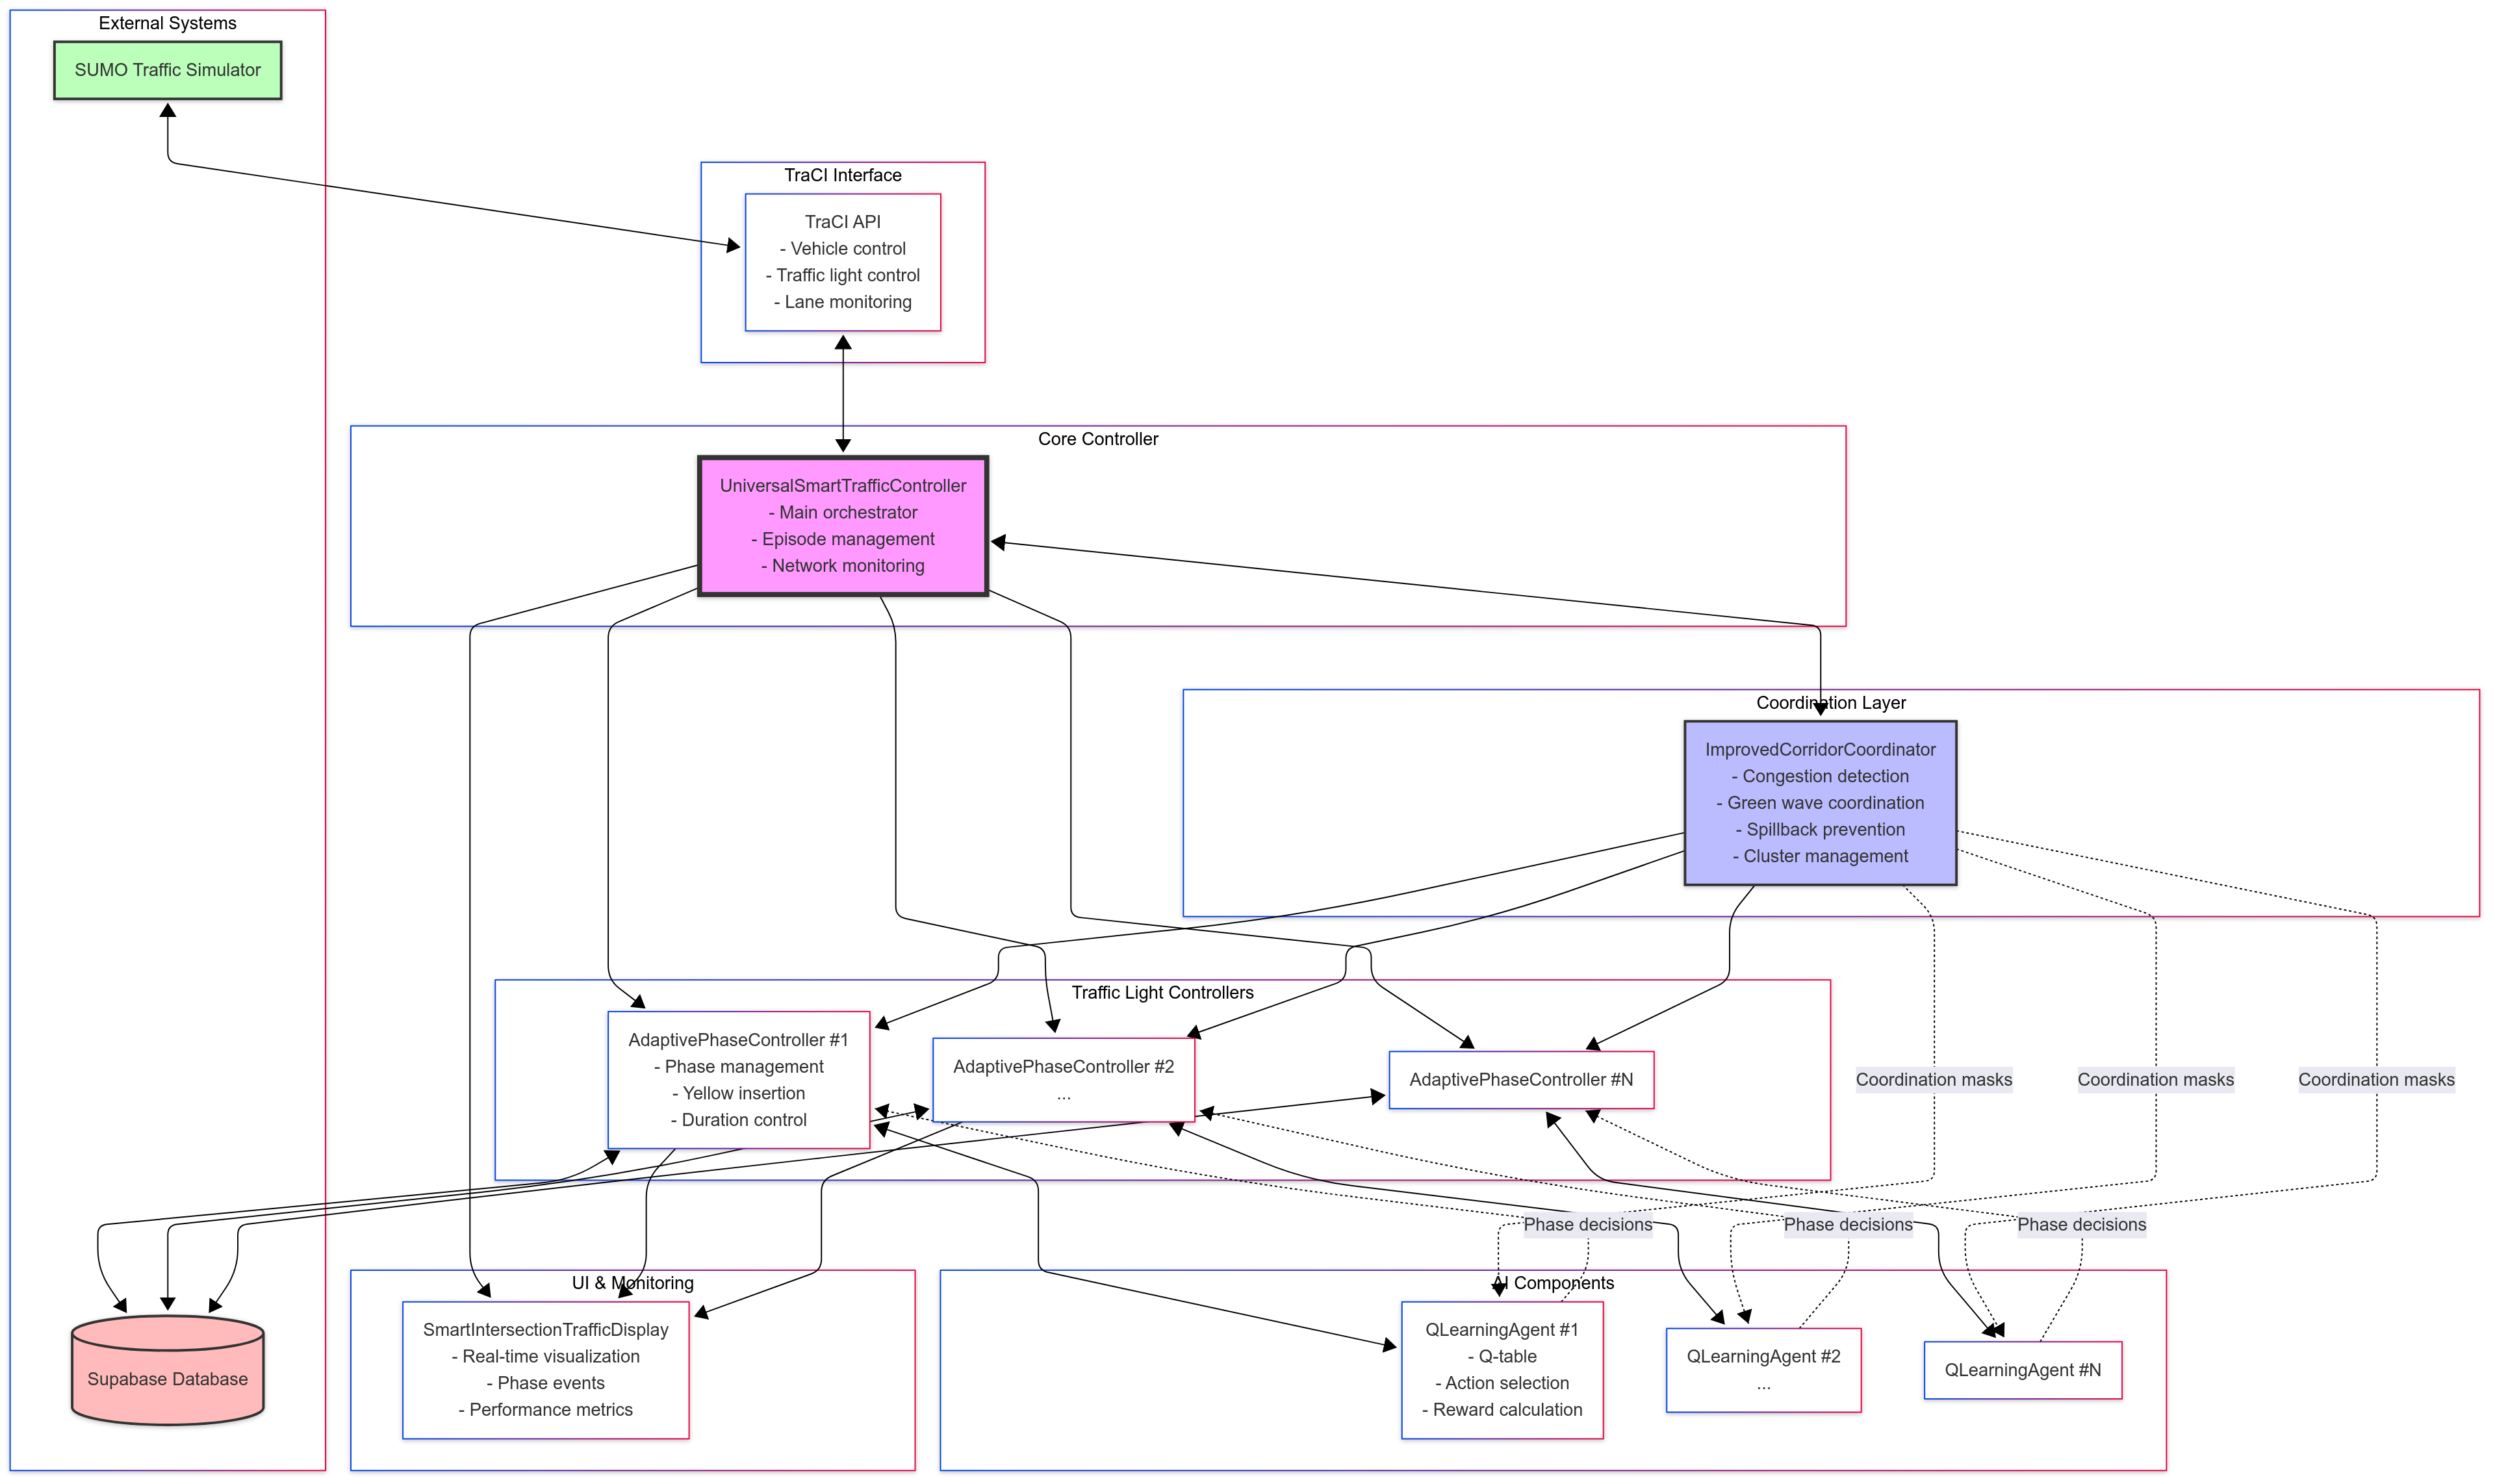
\includegraphics[width=1\linewidth]{Untitled diagram _ Mermaid Chart-2025-08-21-023904.png}

    
    \caption{Kiến trúc tổng thể hệ thống điều khiển đèn giao thông thông minh}
    \label{fig:system_architecture}
\end{figure}

Hệ thống bao gồm 4 tầng chính:

\textbf{Tầng mô phỏng (Simulation Layer):} SUMO đóng vai trò là môi trường mô phỏng giao thông vi mô (microscopic), cung cấp dữ liệu thời gian thực về trạng thái các phương tiện, làn đường và tín hiệu đèn. Đây là nền tảng để kiểm thử và đánh giá hiệu năng của các thuật toán điều khiển trong điều kiện giao thông đa dạng.

\textbf{Tầng giao tiếp (Interface Layer):} TraCI (Traffic Control Interface) đóng vai trò cầu nối hai chiều giữa SUMO và hệ thống điều khiển Python. TraCI cho phép đọc trạng thái mô phỏng thông qua subscription mechanism và gửi lệnh điều khiển đèn tín hiệu theo từng bước thời gian với các wrapper function đảm bảo an toàn.

\textbf{Tầng điều khiển (Control Layer):} Lõi của hệ thống với kiến trúc phân cấp: UniversalSmartTrafficController làm bộ điều khiển trung tâm, quản lý nhiều AdaptivePhaseController (mỗi APC phụ trách một nút giao). Mỗi APC tích hợp với EnhancedQLearningAgent để ra quyết định tối ưu. Đặc biệt, ImprovedCorridorCoordinator điều phối nhiều nút giao, phát hiện cụm tắc nghẽn và tạo green wave cho tuyến đường chính.

\textbf{Tầng lưu trữ (Storage Layer):} Hệ thống hybrid với hai thành phần: (1) Supabase cung cấp cơ sở dữ liệu đám mây để lưu trữ trạng thái APC, lịch sử điều chỉnh pha và nhật ký sự kiện với cơ chế batch write và retry logic; (2) Local storage lưu Q-table trong file pickle để đảm bảo hiệu suất truy xuất nhanh trong quá trình học. SmartIntersectionTrafficDisplay cung cấp giao diện giám sát real-time và phân tích metrics.
\subsection{Luồng dữ liệu}

Luồng dữ liệu trong hệ thống hoạt động theo chu trình closed-loop:

\begin{enumerate}
    \item \textbf{Thu thập dữ liệu:} TraCI đọc trạng thái giao thông từ SUMO, bao gồm số lượng xe, tốc độ trung bình, hàng chờ và thời gian chờ trên mỗi làn đường.
    
    \item \textbf{Xử lý và phân tích:} UniversalSmartTrafficController tổng hợp dữ liệu từ tất cả các làn đường, tính toán các chỉ số hiệu suất như mật độ, lưu lượng và mức độ tắc nghẽn.
    
    \item \textbf{Ra quyết định:} AdaptivePhaseController kết hợp với QLearningAgent để đưa ra quyết định chuyển pha hoặc điều chỉnh thời lượng dựa trên trạng thái hiện tại và kinh nghiệm học được.
    
    \item \textbf{Thực thi điều khiển:} Lệnh điều khiển được gửi ngược lại SUMO thông qua TraCI để thay đổi trạng thái đèn tín hiệu.
    
    \item \textbf{Lưu trữ và học:} Kết quả hành động và phần thưởng được lưu vào Supabase, cập nhật Q-table để cải thiện quyết định trong tương lai.
\end{enumerate}

\subsection{Các điểm tích hợp}

Hệ thống được thiết kế với nhiều điểm tích hợp linh hoạt:

\textbf{TraCI API:} Cung cấp hơn 100 hàm API để tương tác với SUMO, từ đọc thông tin cơ bản đến điều khiển phức tạp. Các subscription được sử dụng để tối ưu băng thông, chỉ lấy dữ liệu cần thiết.

\textbf{Supabase REST API:} Cho phép đồng bộ dữ liệu không đồng bộ với cơ sở dữ liệu đám mây, hỗ trợ batch insert để giảm độ trễ và tăng throughput.

\textbf{Corridor Coordinator Interface:} Module ImprovedCorridorCoordinator cung cấp khả năng điều phối nhiều nút giao, phát hiện cụm tắc nghẽn và tối ưu hóa luồng giao thông trên toàn mạng lưới.

\section{Các thành phần cốt lõi}

\subsection{Bộ điều khiển giao thông thông minh tổng quát}

UniversalSmartTrafficController là thành phần điều khiển cấp cao nhất, chịu trách nhiệm:

\begin{itemize}
    \item \textbf{Quản lý đa nút giao:} Khởi tạo và quản lý nhiều AdaptivePhaseController, mỗi bộ điều khiển phụ trách một nút giao thông độc lập.
    
    \item \textbf{Thu thập dữ liệu toàn cục:} Tổng hợp thông tin từ tất cả các làn đường trong mạng lưới thông qua lane subscription với TraCI.
    
    \item \textbf{Phân tích mạng lưới:} Xác định làn rẽ trái/phải, phát hiện tuyến đường chính (arterial), tính toán mức độ nghẽn cho từng khu vực.
    
    \item \textbf{Điều phối chiến lược:} Kích hoạt chế độ ưu tiên khẩn cấp, chế độ chống tắc nghẽn toàn cục, và điều phối green wave cho tuyến chính.
\end{itemize}

Controller duy trì các cấu trúc dữ liệu quan trọng như \texttt{lane\_to\_tl} (ánh xạ làn-đèn), \texttt{tl\_action\_sizes} (số pha mỗi đèn), và \texttt{intersection\_data} (dữ liệu thời gian thực).

\subsection{Bộ điều khiển pha thích nghi (APC)}

AdaptivePhaseController thực hiện điều khiển cấp nút giao với các chức năng:

\textbf{Điều chỉnh pha động:} Module \texttt{adjust\_phase\_duration()} tính toán thời lượng pha tối ưu dựa trên hàng chờ, thời gian chờ và mật độ giao thông. Công thức điều chỉnh:
\[
\Delta t = \alpha \cdot (R - R_{target})
\]
trong đó $R$ là phần thưởng hiện tại, $R_{target}$ là mục tiêu động, và $\alpha$ là hệ số học.

\textbf{Quản lý pha đèn vàng:} Hàm \texttt{insert\_yellow\_phase\_if\_needed()} tự động chèn pha vàng an toàn khi chuyển từ xanh sang đỏ, với thời lượng thích ứng theo tốc độ phương tiện và chiều dài hàng chờ.

\textbf{Xử lý rẽ trái bảo vệ:} Module \texttt{detect\_blocked\_left\_turn\_with\_conflict()} phát hiện làn rẽ trái bị chặn và kích hoạt pha bảo vệ riêng để giải phóng.

\textbf{Ưu tiên khẩn cấp:} Hệ thống hàng đợi ưu tiên \texttt{pending\_requests} quản lý các yêu cầu chuyển pha theo mức độ ưu tiên: emergency > critical\_starvation > heavy\_congestion > normal.

\subsection{Tác tử Q-learning cải tiến}

EnhancedQLearningAgent triển khai thuật toán học tăng cường với các cải tiến:

\textbf{Không gian trạng thái:} Vector 12 chiều mã hóa thông tin giao thông toàn diện:
\begin{itemize}
    \item Chỉ số hàng chờ (max, mean)
    \item Tốc độ phương tiện (min, mean)  
    \item Thời gian chờ (max, mean)
    \item Pha hiện tại và tổng số pha
    \item Hàng chờ làn rẽ trái/phải
\end{itemize}

\textbf{Cơ chế học thích ứng:} Tham số epsilon giảm dần theo \texttt{epsilon\_decay}, cân bằng giữa khám phá và khai thác. Optimistic initialization với giá trị 10.0 khuyến khích khám phá pha mới.

\textbf{Hàm thưởng đa mục tiêu:} Kết hợp nhiều yếu tố với trọng số thích ứng:
\[
R = 100 \cdot (-w_q \cdot Q + w_v \cdot V - w_w \cdot W - w_d \cdot D + bonus - penalty)
\]

\textbf{Tích hợp Coordinator:} Agent có thể nhận mask từ ImprovedCorridorCoordinator để hạn chế không gian hành động, đảm bảo phối hợp toàn cục.

\subsection{Lớp giao tiếp SUMO--TraCI}

TraCI Interface cung cấp abstraction layer cho việc tương tác với SUMO:

\textbf{Subscription Management:} Đăng ký theo dõi các biến quan trọng của làn đường và phương tiện, giảm overhead communication.

\textbf{Safe Phase Control:} Các wrapper function như \texttt{safe\_set\_phase()} và \texttt{\_safe\_phase\_index()} đảm bảo chỉ số pha luôn hợp lệ, tránh crash.

\textbf{Logic Cache:} Cache logic đèn tín hiệu với TTL 0.5s, giảm số lần query và tăng hiệu suất.

\section{Công nghệ sử dụng}

\subsection{Môi trường Python}

Hệ thống được phát triển với Python 3.8+, tận dụng các tính năng hiện đại:

\begin{itemize}
    \item \textbf{Async/Await:} Xử lý I/O không đồng bộ với Supabase
    \item \textbf{Type Hints:} Tăng độ tin cậy và khả năng bảo trì code
    \item \textbf{Dataclasses:} Quản lý cấu trúc dữ liệu phức tạp
    \item \textbf{Threading:} Chạy parallel cho database writer và display
\end{itemize}

\subsection{Mô phỏng giao thông SUMO}

SUMO (Simulation of Urban MObility) version 1.22.0 cung cấp:

\begin{itemize}
    \item \textbf{Microscopic simulation:} Mô phỏng từng phương tiện riêng lẻ
    \item \textbf{Network editor:} Công cụ NETEDIT để thiết kế mạng lưới
    \item \textbf{Demand generation:} Tạo luồng giao thông thực tế
    \item \textbf{Output analysis:} Xuất dữ liệu chi tiết để đánh giá
\end{itemize}

\subsection{Tích hợp API TraCI}

TraCI 1.22.0 cung cấp Python binding với các module chính:

\begin{itemize}
    \item \texttt{traci.trafficlight}: Điều khiển đèn tín hiệu
    \item \texttt{traci.lane}: Đọc thông tin làn đường
    \item \texttt{traci.vehicle}: Theo dõi phương tiện
    \item \texttt{traci.simulation}: Quản lý mô phỏng
\end{itemize}

\subsection{Cấu hình Supabase}

Supabase cung cấp cơ sở dữ liệu PostgreSQL được quản lý trên đám mây với khả năng real-time và REST API tự động. Hệ thống sử dụng 4 bảng chính với cấu trúc được tối ưu cho việc lưu trữ và truy vấn dữ liệu giao thông:

\subsubsection{Bảng apc\_states}

Bảng chính lưu trữ trạng thái đầy đủ của các bộ điều khiển APC (Adaptive Phase Controller):

\begin{figure}[H]
    \centering
    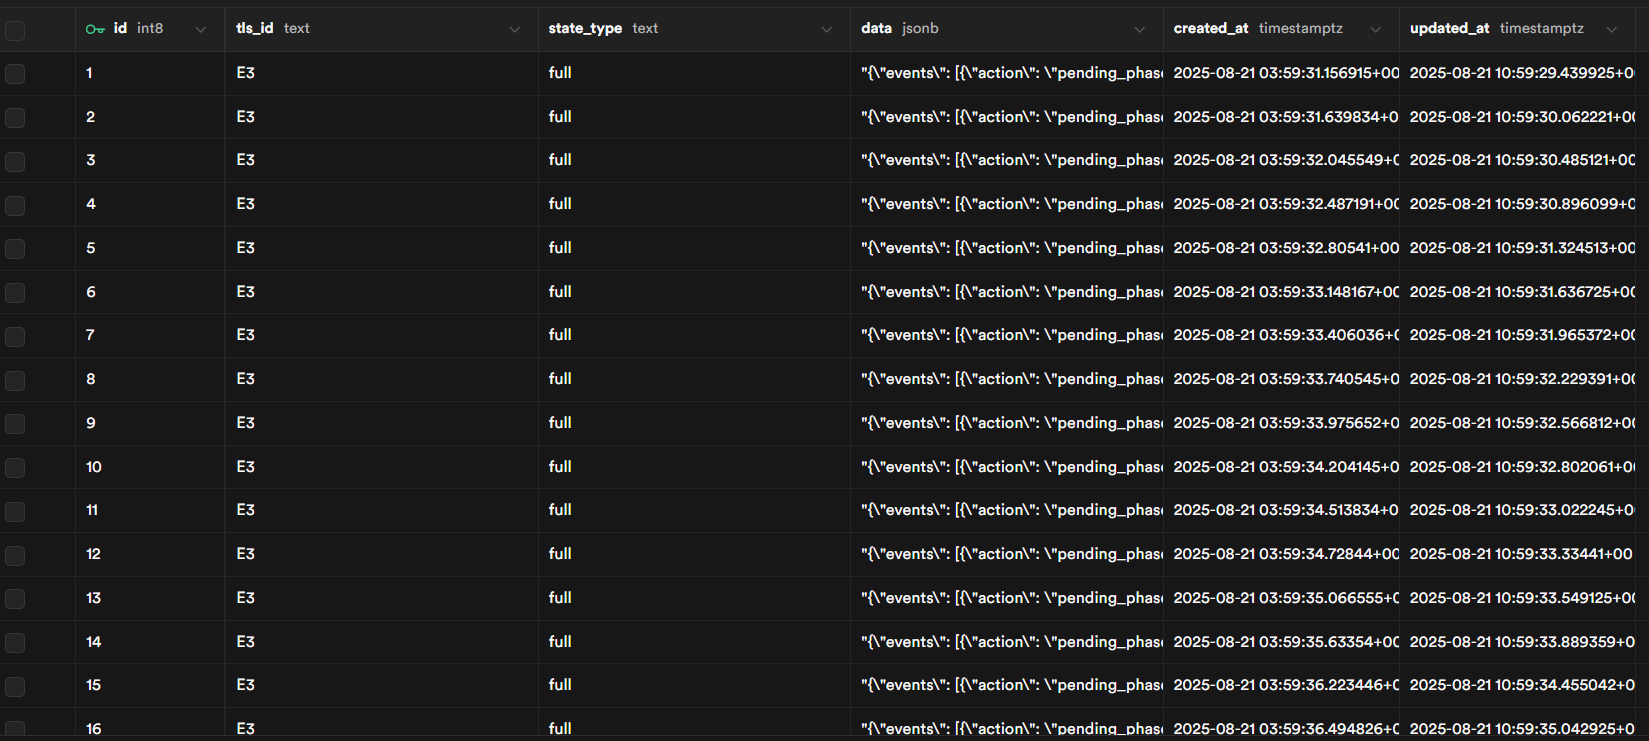
\includegraphics[width=1\linewidth]{tut.png}
    \caption{Dữ liệu mẫu trong bảng apc\_states}
    \label{fig:apc_states_data}
\end{figure}

Bảng \texttt{apc\_states} được thiết kế với cấu trúc linh hoạt để lưu trữ nhiều loại trạng thái khác nhau của hệ thống điều khiển:

\begin{lstlisting}[style=sql,caption={Định nghĩa cấu trúc bảng apc\_states}]
CREATE TABLE apc_states (
    id BIGSERIAL PRIMARY KEY,
    tls_id TEXT NOT NULL,           -- ID của nút giao thông
    state_type TEXT NOT NULL,       -- Loại trạng thái
    data JSONB NOT NULL,            -- Dữ liệu trạng thái
    created_at TIMESTAMPTZ DEFAULT NOW(),
    updated_at TIMESTAMPTZ DEFAULT NOW()
);

-- Tạo index để tối ưu truy vấn
CREATE INDEX idx_apc_states_tls_type 
    ON apc_states(tls_id, state_type);
CREATE INDEX idx_apc_states_data 
    ON apc_states USING gin(data);
\end{lstlisting}

Trường \texttt{state\_type} phân loại dữ liệu thành ba nhóm chính:

\begin{itemize}
    \item \textbf{\texttt{full}}: Snapshot toàn bộ trạng thái APC tại một thời điểm, bao gồm:
        \begin{itemize}
            \item Cấu hình các pha đèn (phase configurations)
            \item Hàng đợi sự kiện đang chờ xử lý
            \item Thông số điều khiển hiện tại
            \item Trạng thái của Q-learning agent
        \end{itemize}
    
    \item \textbf{\texttt{phase}}: Thông tin chi tiết về một pha đèn cụ thể:
        \begin{itemize}
            \item Thời lượng thực tế và cơ sở
            \item Danh sách làn đường được phục vụ
            \item Điều chỉnh thời gian ($\Delta t$)
        \end{itemize}
    
    \item \textbf{\texttt{event}}: Sự kiện điều khiển đơn lẻ:
        \begin{itemize}
            \item Chuyển pha khẩn cấp
            \item Kích hoạt rẽ trái bảo vệ
            \item Phát hiện tắc nghẽn
        \end{itemize}
\end{itemize}

Việc sử dụng JSONB cho trường \texttt{data} mang lại nhiều lợi ích:
- Linh hoạt trong việc mở rộng cấu trúc dữ liệu
- Hỗ trợ query và indexing hiệu quả với GIN index
- Dễ dàng tích hợp với Python thông qua JSON serialization

\subsubsection{Bảng phase\_records}

Lưu trữ lịch sử chi tiết về mọi điều chỉnh pha trong hệ thống:

\begin{table}[H]
\centering
\footnotesize
\begin{tabular}{|l|l|p{6cm}|}
\hline
\textbf{Cột} & \textbf{Kiểu dữ liệu} & \textbf{Mô tả} \\
\hline
\hline
\multicolumn{3}{|c|}{\textit{Thông tin cơ bản}} \\
\hline
id & BIGSERIAL & Khóa chính tự tăng \\
tls\_id & TEXT & ID của nút giao thông \\
phase\_idx & INTEGER & Chỉ số pha (0-11) \\
sim\_time & REAL & Thời điểm trong mô phỏng (giây) \\
\hline
\multicolumn{3}{|c|}{\textit{Thông số thời gian}} \\
\hline
duration & REAL & Thời lượng thực tế của pha (giây) \\
base\_duration & REAL & Thời lượng cơ sở theo cấu hình \\
delta\_t & REAL & Mức điều chỉnh sau làm mượt \\
raw\_delta\_t & REAL & Mức điều chỉnh ban đầu \\
extended\_time & REAL & Thời gian mở rộng thêm \\
\hline
\multicolumn{3}{|c|}{\textit{Thông tin điều khiển}} \\
\hline
state\_str & TEXT & Chuỗi trạng thái (vd: "GGrrGGrr") \\
event\_type & TEXT & Loại sự kiện kích hoạt điều chỉnh \\
weights & JSONB & Trọng số các yếu tố điều khiển \\
lanes & JSONB & Danh sách làn đường được phục vụ \\
\hline
\multicolumn{3}{|c|}{\textit{Đánh giá hiệu suất}} \\
\hline
reward & REAL & Phần thưởng từ RL agent \\
penalty & REAL & Hình phạt cho điều chỉnh quá mức \\
bonus & REAL & Điểm thưởng cho hiệu suất tốt \\
\hline
\multicolumn{3}{|c|}{\textit{Metadata}} \\
\hline
created\_at & TIMESTAMPTZ & Thời điểm tạo bản ghi \\
updated\_at & TIMESTAMPTZ & Thời điểm cập nhật cuối \\
\hline
\end{tabular}
\caption{Cấu trúc chi tiết bảng phase\_records với phân nhóm theo chức năng}
\label{tab:phase_records_detailed}
\end{table}

Bảng này đóng vai trò quan trọng trong việc:
\begin{itemize}
    \item Theo dõi lịch sử điều chỉnh để phân tích hiệu suất
    \item Cung cấp dữ liệu huấn luyện cho Q-learning agent
    \item Phát hiện các pattern giao thông lặp lại
    \item Debug và tối ưu hóa thuật toán điều khiển
\end{itemize}

\subsubsection{Bảng simulation\_events}

Ghi nhận mọi sự kiện trong quá trình mô phỏng:

\begin{figure}[H]
    \centering
    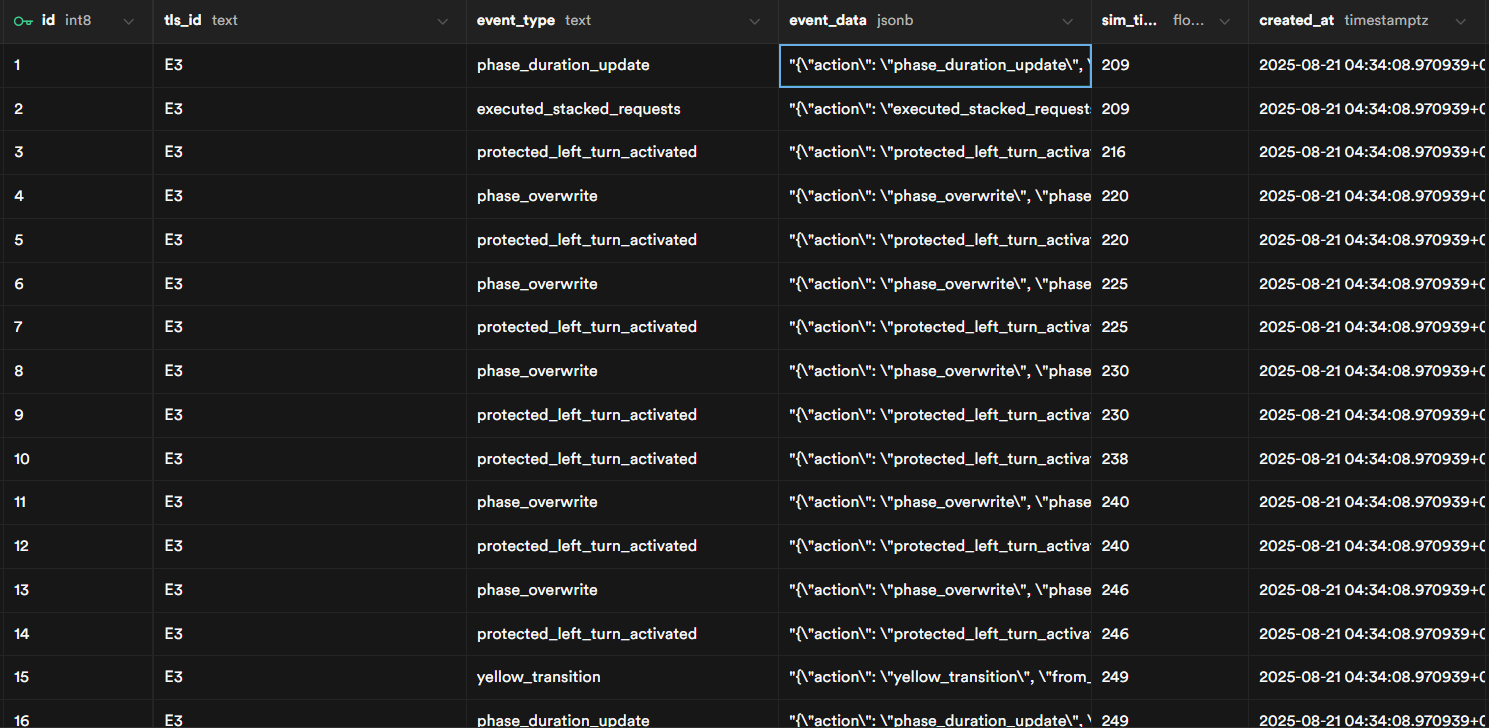
\includegraphics[width=1\linewidth]{TUTU.png}
    \caption{Dữ liệu thực tế từ bảng simulation\_events}
    \label{fig:simulation_events_data}
\end{figure}

Bảng \texttt{simulation\_events} (Hình \ref{fig:simulation_events_data}) lưu trữ lịch sử chi tiết các sự kiện điều khiển đèn giao thông với cấu trúc:

\begin{itemize}
    \item \texttt{id}: Khóa chính tự tăng (int8)
    \item \texttt{tls\_id}: ID của đèn giao thông (text) - trong ví dụ là "E3"
    \item \texttt{event\_type}: Loại sự kiện điều khiển (text)
    \item \texttt{event\_date}: Dữ liệu JSON chứa chi tiết sự kiện (jsonb)
    \item \texttt{sim\_time}: Thời điểm trong mô phỏng (float)
    \item \texttt{created\_at}: Thời điểm tạo bản ghi (timestamptz)
\end{itemize}

Ví dụ cấu trúc dữ liệu JSON trong cột \texttt{event\_date}:

\begin{lstlisting}[style=json,caption={Cấu trúc JSON của sự kiện phase\_duration\_update}]
{
    "action": "phase_duration_update",
    "phase": 209
}
\end{lstlisting}

\begin{lstlisting}[style=json,caption={Cấu trúc JSON của sự kiện phase\_overwrite}]
{
    "action": "phase_overwrite", 
    "phase": 220
}
\end{lstlisting}

Các loại sự kiện chính được ghi nhận trong hệ thống:
\begin{itemize}
    \item \texttt{phase\_duration\_update}: Cập nhật thời lượng pha đèn động
    \item \texttt{executed\_stacked\_requests}: Thực thi các yêu cầu đã được xếp hàng đợi
    \item \texttt{protected\_left\_turn\_activated}: Kích hoạt pha rẽ trái được bảo vệ
    \item \texttt{phase\_overwrite}: Ghi đè pha hiện tại với cấu hình mới
    \item \texttt{yellow\_transition}: Chuyển sang pha đèn vàng an toàn
\end{itemize}

Dữ liệu trong bảng cho thấy hệ thống liên tục điều chỉnh hoạt động, với các sự kiện được ghi nhận theo thời gian thực. Đặc biệt, sự kiện \texttt{protected\_left\_turn\_activated} xuất hiện nhiều lần (8/16 bản ghi), cho thấy hệ thống thường xuyên phải xử lý tình huống rẽ trái phức tạp tại nút giao này.


\subsubsection{Tối ưu hiệu suất database}

Hệ thống áp dụng nhiều kỹ thuật tối ưu:

\textbf{Indexing chiến lược:} Tạo composite index cho các truy vấn thường xuyên:
\begin{lstlisting}[style=sql]
CREATE INDEX idx_apc_states_tls_type 
    ON apc_states(tls_id, state_type);
CREATE INDEX idx_phase_records_phase_idx 
    ON phase_records(tls_id, phase_idx);
\end{lstlisting}

\textbf{JSONB cho flexibility:} Sử dụng JSONB thay vì JSON thuần để có khả năng index và query hiệu quả với GIN index.

\textbf{Row Level Security (RLS):} Bảo mật ở cấp độ row với policy:
\begin{lstlisting}[style=sql]
ALTER TABLE apc_states ENABLE ROW LEVEL SECURITY;
CREATE POLICY "Enable all operations for authenticated users" 
    ON apc_states
    FOR ALL USING (auth.role() = 'authenticated');
\end{lstlisting}

\textbf{Batch operations:} Module PatchedAsyncSupabaseWriter thực hiện batch insert với kích thước tối đa 100 records và interval 60 giây, giảm số lượng round-trip đến database.

\subsubsection{Chiến lược đồng bộ dữ liệu}

Hệ thống sử dụng mô hình write-behind cache:

\begin{enumerate}
    \item \textbf{Buffer cục bộ:} Dữ liệu được tích lũy trong \texttt{\_pending\_db\_ops} với giới hạn \texttt{MAX\_PENDING\_DB\_OPS = 1000}
    
    \item \textbf{Flush định kỳ:} AsyncSupabaseWriter flush dữ liệu mỗi 60 giây hoặc khi buffer đầy
    
    \item \textbf{Retry logic:} Exponential backoff với max 6 lần retry cho mỗi batch
    
    \item \textbf{Graceful degradation:} Nếu Supabase không khả dụng, hệ thống vẫn hoạt động với local cache
\end{enumerate}

Thiết kế này đảm bảo hệ thống có thể xử lý hàng triệu events mỗi giờ mà không ảnh hưởng đến hiệu suất real-time của điều khiển giao thông.

Hệ thống sử dụng các thư viện Python sau:

\begin{itemize}
    \item \textbf{NumPy 1.24+:} Tính toán ma trận và vector hiệu suất cao
    \item \textbf{Pandas 2.0+:} Xử lý và phân tích dữ liệu dạng bảng
    \item \textbf{Matplotlib 3.7+:} Trực quan hóa kết quả mô phỏng
    \item \textbf{Supabase-py 2.4+:} Client SDK cho Supabase
    \item \textbf{Threading, Queue:} Xử lý đa luồng và hàng đợi
    \item \textbf{Pickle:} Serialize/deserialize Q-table
\end{itemize}

Kiến trúc module này đảm bảo hệ thống có khả năng mở rộng, dễ bảo trì và hiệu suất cao trong việc điều khiển giao thông thông minh.
